\documentclass[a4paper,10pt]{article}
\usepackage[utf8]{inputenc}
\usepackage{graphicx}
\usepackage{amssymb}
\usepackage{amsmath}

%opening
\author{Emmanuel Peto Gutiérrez}
\title{Inteligencia Artificial Examen 2\\2023-I}

\begin{document}

\maketitle

\paragraph{Intrucciones:} Para cada problema conteste lo que se le pide.

 \begin{enumerate}
 \item \textbf{(3 puntos) Considere la red Bayesiana de la imagen y conteste lo siguiente}
	\begin{itemize}
		\item \textbf{(1 puntos) ¿Cuál de las siguientes redes se establece por la red?}

Respuesta: la que está subrayada.

		\begin{itemize}
			\item $P(B,I,M)=P(B)P(I)P(M)$
			
			\item  \underline{$P(J| G)=P(J | G,I)$}
			
			\item $P(M| G,B,I)=p(M| G,B,I,J)$
			
		\end{itemize}

		\item \textbf{(1 puntos) Calcular el valor de} $P(b,i,m,g,j)$

Nota: se va a interpretar $P(b,i,m,g,j)$ como $P(B:t, I:t, M:t, G:t, J:t)$.

$P(b,i,m,g,j)$\\
$= P(b,m,i,g,j)$\\
$= P(b) P(m) P(i | m,b) P(g | b,m,i) P(j | g)$\\
$= 0.9 \times 0.1 \times 0.9 \times 0.9 \times 0.9$\\
\underline{$= 0.06561$}

		\item \textbf{(1 puntos) Calcular la probabilidad de que alguien vaya a la carcel dado que rompieron la ley, han sido acusados y tienen a un fiscal políticamente motivado.}

% $P(j | b,g,m) = P(j | g)$, porque $j$ sólo depende de $g$. Así que \underline{$P(j | b,g,m) = 0.9$}.

Se requiere calcular $P(j | b, g, m)$. Por definición de probabilidad condicional se tiene que $P(j | b, g, m) = \frac{P(j, b, g, m)}{P(b, g, m)}$. Así que hay que calcular las probabilidades en el cociente.

$\bullet P(j, b, g, m) = P(j, b, g, m, I:t) + P(j, b, g, m, I:f)$.

$\bullet P(j, b, g, m, I:1) = 0.06561$ (obtenido en el inciso anterior).

$\bullet P(j, b, g, m, I:0) = P(b)P(m)P(I:f | m, b) P(g | b, m, I:f) P(j | g) = 0$ (porque $P(g | b, m, I:f) = 0$)

Por lo tanto $P(j, b, g, m) = 0.06561$.

Luego

$\bullet P(b, g, m) = P(b, g, m, I:t, J:t) + P(b, g, m, I:f, J:t) + P(b, g, m, I:t, J:f) + P(b, g, m, I:f, J:f)$

$\bullet P(b, g, m, I:t, J:t) = P(b) P(m) P(I:t | m,b) P(g | b,m,I:t) P(J:t | g) = 0.06561$

$\bullet P(b, g, m, I:f, J:t) = P(b) P(m) P(I:f | m,b) P(g | b,m,I:f) P(J:t | g) = 0$ (porque $P(g | b,m,I:f) = 0$)

$\bullet P(b, g, m, I:t, J:f) = P(b) P(m) P(I:t | m,b) P(g | b,m,I:t) P(J:f | g) = 0.9 \times 0.1 \times 0.9 \times 0.9 \times 0.1 = 0.00729$

$\bullet P(b, g, m, I:f, J:f) = P(b) P(m) P(I:f | m,b) P(g | b,m,I:f) P(J:f | g) = 0$

Entonces $P(b, g, m) = 0.06561 + 0.00729 = 0.0729$.

Retomando la definición de probabilidad condicional, se tiene $P(j | b, g, m) = \frac{0.06561}{0.0729} = 0.9$.

	\end{itemize}
    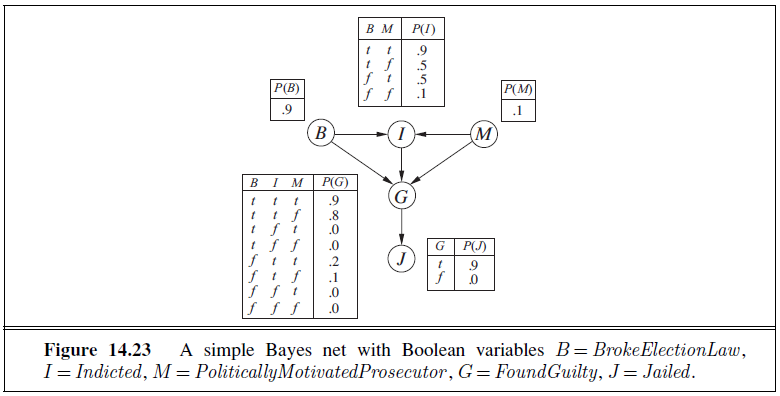
\includegraphics[width=\textwidth]{img7}

 \item (3 puntos) \textbf{Suponga que tenemos un conjunto de datos con cinco predictores}
 \begin{itemize}
  \item $X_1=$ \textbf{Promedio (entre 0 y 4.0)}
  \item $X_2=$ \textbf{IQ}
  \item $X_3=$ \textbf{Nivel educativo (1 universidad y 0 preparatoria)}
  \item $X_4= X_1X_2$ 
  \item $X_5= X_1X_3$ 
 \end{itemize}

 \textbf{La respuesta es el salario después de graduarse (en miles)}
  \textbf{Suponga que se usa minimos cuadrados para ajustar el modelo y se obtiene:} $\hat\beta_0=50, \hat\beta_1=20, \hat\beta_2=0.07, \hat\beta_3=35, \hat\beta_4=0.01, \hat\beta_5=-10$
  \begin{enumerate}
   \item \textbf{(2 puntos) ¿Cuál respuesta es correcta y por qué?}

La respuesta es la subrayada. Tómense los valores fijos $X_1 = p$, $X_2 = i$. Entonces se tienen las siguientes ecuaciones para salario de prepa ($sp$) y salario de universidad ($su$):

$sp = 50 + 20p + 0.07i + 0.01pi$

$su = 50 +20p + 0.07i + 35 + 0.01pi - 10p$

Restando ambas ecuaciones se tiene que $su - sp = 35 - 10p$. Si $su - sp > 0$ significa que el salario de universidad es mayor que el de prepa; si $su - sp < 0$ significa que el salario de prepa es mayor que el de universidad. Entonces $35 - 10p < 0$ si $p$ es lo suficientemente alto; en particular, si $p > 3.5$. Por lo tanto, cuando $p > 3.5$, el salario de un graduado de prepa será mayor que el de un graduado de universidad.

    \begin{enumerate}
        \item Para un valor fijo de IQ y promedio, los graduados de preparatoria ganan más en promedio que los graduados de universidad
        \item Para un valor fijo de IQ y promedio, los graduados de universidad ganan más en promedio que los graduados de preparatoria
        \item \underline{Para un valor fijo de IQ y promedio, los graduados de preparatoria} \underline{ganan más en promedio que los graduados de universidad si el promedio} \underline{es suficientemente alto}
        \item Para un valor fijo de IQ y promedio, los graduados de universidad ganan más en promedio que los graduados de preparatoria
        el promedio es suficientemente alto
    \end{enumerate}
    \item \textbf{(1 punto) Predecir el salario de un graduado de universidad con IQ de 110 y un promedio de 4.0}
    
$salario(X_1, X_2, X_3, X_4, X_5)$\\
$= salario(4, 110, , 440, 4)$\\
$= 50 + 20(4) + 0.07(110) + 35(1) + 0.01(440) - 10(4)$\\
$= 137.1$

Y como el resultado de la función está en miles, entonces su sueldo estimado sería \underline{137,100} pesos.

  \end{enumerate}

  \item \textbf{(3 puntos) Suponga que se recolectan datos de un grupo de estudiantes de inteligencia artificial con las variables:}
  \begin{itemize}
   \item $X_1=$ \textbf{horas de estudio}
   \item $X_2=$ \textbf{promedio en otros cursos}
  \end{itemize}
  \textbf{y la respuesta, calificación de 4. Al ajustar el modelo de regresión logística los coeficientes fueron:} $\hat\beta_0=-6, \hat\beta_1=0.05,\hat\beta_2=1$.
   \begin{enumerate}
    \item \textbf{(1.5 punto) Estimar la probabilidad que un estudiante que estudió 40 horas y tiene un promedio de 3.5 obtenga un 4 en la clase}
    
En este caso, se tomará la variable $y = 1$ si obtiene un 4 o $y = 0$ si no obtiene 4. Sea $\exp(k) = e^k$.

\[p(X) = \frac{1}{1 + \exp (-(\beta_0 + \beta_1 X_1 + \beta_2 X_2))} \]

\[= \frac{1}{1+ \exp (-(-6 +  0.05(40) + 3.5))} \]

\[= \frac{1}{1+ \exp (-(-0.5))} \]

\[= \frac{1}{1+ \exp (0.5)} \]

\[= 0.3775 \]

Entonces la probabilidad es \underline{0.3775}

    \item \textbf{(1.5 punto) ¿Cuántas horas debería estudiar un estudiante con un promedio de 3.5 para tener un 50\% de probabilidad de obtener un 4 en la clase?}
    
Sea $p(x)$ la probabilidad de que $x$ obtenga un 4. Se sabe que en este modelo $\log (\frac{p(x)}{1-p(x)}) = \beta_0 + \beta_1 X_1 + \beta_2 X_2$. Se sabe que $p(x) = 0.5$, entonces $\log (\frac{0.5}{1-0.5}) = \log (\frac{0.5}{0.5}) = \log (1) = 0$.

Entonces $-6 + 0.05t + 3.5 = 0$, donde $t$ es el tiempo que debe estudiar.

$\Rightarrow 0.05t -2.5 = 0$\\
$\Rightarrow 0.05t = 2.5$\\
$\Rightarrow t = 2.5/0.05 = 50$

El estudiante debe estudiar \underline{50 horas}.

   \end{enumerate}
 
	\item \textbf{(3 puntos) considere el problema mostrado en la imagen. Genere la política para los siguientes escenarios considerando un descuento de .99 mediante iteración de valor. Explique intuitivamente la relación entre el valor $r$ y la política}

    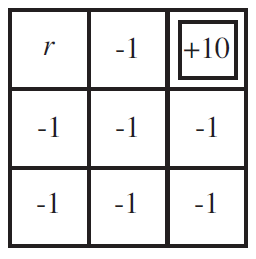
\includegraphics[width=0.4\textwidth]{img8}

Para este problema se harán las siguientes consideraciones: el agente no puede empezar en la casilla que contiene a $r$ ni en la que contiene a +10. No se puede mover en diagonal. Si el agente ya llegó a la casilla que contiene a $r$ o a la que tiene +10, entonces ya no se puede mover (por lo que no habrá política).

	\begin{itemize}
		\item \textbf{(1 punto)  r = 100}
		
Primero se construirá una matriz con pares de números: la primera entrada es el valor de la recompensa al alcanzar $r$ y la segunda entrada es el de la recompensa al alcanzar el 10.

\begin{tabular}{|c|c|c|}
\hline
 & (98, 8.9) & \\ \hline
(98, 6.703) & (96.01, 7.801) & (94.03, 8.9) \\ \hline
(96.01, 5.606) & (94.03, 6.703) & (92.06, 7.801) \\ \hline
\end{tabular}

La política va a estar definida por el valor más alto de recompensa. En este caso, independientemente de la casilla en la que se inicie, siempre es más conveniente alcanzar $r$ (que vale 100). La tabla de políticas es la siguiente:

\begin{tabular}{|c|c|c|}
\hline
 & $\leftarrow$ & \\ \hline
$\uparrow$ & $\leftarrow$ & $\leftarrow$ \\ \hline
$\uparrow$ & $\leftarrow$ & $\leftarrow$ \\ \hline
\end{tabular}

		\item \textbf{(1 punto)  r = -3}
		
Matriz de recompensas:

\begin{tabular}{|c|c|c|}
\hline
 & (-3.97, 8.9) & \\ \hline
(-3.97, 6.703) & (-4.9403, 7.801) & (-5.911, 8.9) \\ \hline
(-4.9403, 5.6069) & (-5.911, 6.703) & (-6.882, 7.801) \\ \hline
\end{tabular}

Matriz de políticas:

\begin{tabular}{|c|c|c|}
\hline
 & $\rightarrow$ & \\ \hline
$\rightarrow$ & $\rightarrow$ & $\uparrow$ \\ \hline
$\rightarrow$ & $\rightarrow$ & $\uparrow$ \\ \hline
\end{tabular}

		\item \textbf{(0.5 punto) r = 0}
		
Matriz de recompensas:

\begin{tabular}{|c|c|c|}
\hline
& (-1.0, 8.9) & \\ \hline
(-1.0, 6.73) & (-2.0, 7.801) & (-3.0, 8.9) \\ \hline
(-2.0, 5.606) & (-3.0, 6.703) & (-4.0, 7.801) \\ \hline
\end{tabular}

Matriz de políticas:

\begin{tabular}{|c|c|c|}
\hline
 & $\rightarrow$ & \\ \hline
$\rightarrow$ & $\rightarrow$ & $\uparrow$ \\ \hline
$\rightarrow$ & $\rightarrow$ & $\uparrow$ \\ \hline
\end{tabular}

		\item \textbf{(0.5 punto) r = +3}
	\end{itemize}

Matriz de recompensas

\begin{tabular}{|c|c|c|}
\hline
& (1.97, 8.9) & \\ \hline
(1.97, 6.703) & (0.9403, 7.801) & (-0.0891, 8.9) \\ \hline
(0.9403, 5.606) & (-0.0891, 6.703) & (-1.118, 7.801) \\ \hline
\end{tabular}

Matriz de políticas

\begin{tabular}{|c|c|c|}
\hline
 & $\rightarrow$ & \\ \hline
$\rightarrow$ & $\rightarrow$ & $\uparrow$ \\ \hline
$\rightarrow$ & $\rightarrow$ & $\uparrow$ \\ \hline
\end{tabular}

    \item \textbf{(0.5 puntos) Opinión del curso}
    \begin{itemize}
     \item \textbf{¿Qué salió bien?}
     
     Terminó a tiempo, respetando el calenario establecido desde el principio. Se nota que domina el tema. Prepara su clase con anticipación. Aprendí sobre cosas que nunca había visto, en realidad conocía poco sobre IA. Se dieron asesorías personalizadas sobre programación. Nos da la opción de tomar la clase desde casa o en el salón.

     \item \textbf{¿Qué se puede mejorar?}
     
     Ir más despacio (aunque quizá así ya no se cumpla el requisito de terminar a tiempo). Publicar las presentaciones en pdf (los usuarios de Linux estaremos agradecidos).
     
     \item \textbf{¿Qué acciones se pueden tomar para mejorar?}
     
     Darnos asesorías sobre probabilidad y estadística. Cortar el temario.

    \end{itemize}

 
\end{enumerate}


\end{document}
